\documentclass[9pt]{article}
\usepackage{multicol,caption}
\usepackage{graphicx}
\usepackage{multicol}
\usepackage{wrapfig}
\setlength{\columnseprule}{0.5pt}
\usepackage[english, russian]{babel}
\usepackage[utf8]{inputenc}
\newenvironment{Figure}
{\par\medskip\noindent\minipage{\linewidth}}
{\endminipage\par\medskip}


\usepackage{geometry}
\geometry{portrait, margin=2in}
\hoffset = -110pt
\voffset = -100pt
\textwidth = 530pt
\textheight = 700pt  

  
\begin{document}

\begin{multicols}{2}

Может ли длина суммы этих векторов равняться а) 1998; б)* $\sqrt{1998}$ ?
Ответ на оба вопроса задачи утвердительный. Начнем
построение примера к пункту а). Длина суммы $\vec{OB2} + \vec{OB3} + \vec{OB4}$
 векторов рисунка 2 равна 2. Чтобы построить систему векторов, длина суммы которых равна 3,
помимо шестиугольника рассмотрим пятиугольник (рис.3).

\begin{wrapfigure}{l}{0.25\textwidth}
  \begin{left}
    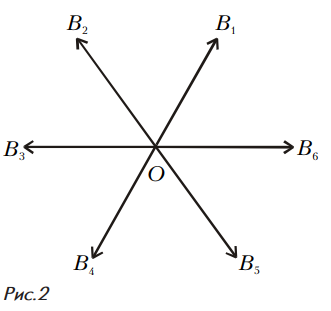
\includegraphics[scale = 0.65]{r2.png}
  \end{left}
\end{wrapfigure}

Благодаря формуле (1)
сумма четырех векторов $\vec{OC_1} + \vec{OC_2} + \vec{OC_3}  + \vec{OC_4}$
, проведенных из центра в четыре вершины правильного пятиугольника,
противоположна вектору $\vec{OC_5}$
, соединяющему центр с пятой вершиной пятиугольника.
И вершины пятиугольника, и вершины шестиугольника лежат в вершинах
правильного 30-угольника.
Аналогично, чтобы построить систему векторов,

\begin{wrapfigure}{l}{0.25\textwidth}
  \begin{left}
    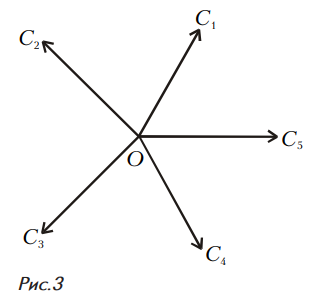
\includegraphics[scale = 0.65]{r3.png}
  \end{left}
\end{wrapfigure}

длина
суммы которых равна 4, добавим еще 6 векторов $\vec{OA_1}$,$\ldots \vec{OA_6}$, соединяющих
центр с вершинами семиугольника (см. рис.1).
Продолжая в таком же
духе, мы и получим пример к пункту а).
Формальное описание
изложенной конструкции
таково. Пусть $n_1, n_2 ,\ldots n_{1998}$ – попарно взаимно простые числа. Рассмотрим правильный $n_1 n_2 \ldots n_{1998}$ -угольник. Зафиксируем некоторую его вершину
A. Назовем «выделенным» $n_i$
-угольником $(i = 1,\ldots 1998)$ правильный $n_i$
-угольник, одной из вершин
которого является точка $A$, а другие вершины являются
вершинами $n_1 n_2 \ldots n_{1998}$ -угольника. Выделенные $n_i$
-угольник и $n_j$
-угольник $(i \neq j)$ имеют, благодаря взаимной
простоте чисел $n_i$
 и $n_j$
, единственную общую вершину $A$.
Рассмотрим векторы, идущие из центра O многоугольника во все вершины всех выделенных $n_i$
-угольников, кроме $A$. Их сумма равна $-1998\vec{OA}$, что и требовалось.
б) В следующем разделе статьи мы построим с привлечением комплексных чисел сумму длиной $\sqrt{n}$ при любом
натуральном $n$, а пока предлагаем ряд упражнений. Тот,
кто справится с ними, получит решение пункта б), не
использующее никаких выходящих за рамки школьной
программы понятий (но, к сожалению, существенно
использующее специфику числа $\sqrt{1998}$ ). \newline
\textbf{Упражнение 1}. Воспользовавшись приемом решения пункта
а), докажите, что если можно представить в искомом виде (т.е.
в виде суммы векторов, проведенных из центра вписанного в
единичную окружность правильного многоугольника в его вершины) некоторый вектор $\vec{v}$, то можно представить в таком виде
и вектор $\vec{av}$, где $a$ – натуральное число. \newline
\textbf{Упражнение 2.} Докажите, что если можно представить в
искомом виде вектор длиной x, то можно представить в таком
виде и вектор длиной а) $x\sqrt{a^2 + b^2}$, б) $x\sqrt{a^2 + 2b^2}$, 
где $a$ и $b$ – натуральные числа.
\emph{Замечание.} Если в искомом виде можно представить некоторый вектор длиной $\sqrt{m}$ , то можно представить и вектор длиной $\sqrt{2m}$ . Поэтому в дальнейшем мы можем искать вектор длиной $\sqrt{n}$ только для нечетных $n$. \newline
\textbf{Упражнение 3.} Решите пункт б) задачи M1648. \newline
\emph{Указание.} $\sqrt{1998}=\sqrt{3^2 + 18^2} \cdot \sqrt{2^2 + 2 \cdot 1^2}$.
\newline
\newline
{\textbf{\large{\qquadКорни из еденицы}}}

Сейчас мы запишем равенство (1) в довольно неожиданном виде. Для этого рассмотрим уравнение $z^n — 1 = 0$ и
разложим его левую часть на множители:
$$(z-1)(z^{n-1}+z^{n-2}+\ldots+z+1)$$
Значит, если $z^n=1$ и $z\neq1$, то \newline
$$z^{n-1}+z^{n-2}+\ldots+z+1=0 \quad(2)$$.
В статье «Многочлены деления круга» («Квант» №1 за
1998 год) рассказано о том, что уравнение $z^n=1$ имеет $n$
решений – «корней из единицы». Они являются вершинами правильного $n$-угольника, вписанного в единичную окружность, и имеют вид
$$\zeta^k=\cos{\frac{2\pi k}{n}}+i\sin{\frac{2\pi k}{n}},$$
где 
$\zeta=\cos{\frac{2\pi}{n}}+i\sin{\frac{2\pi}{n},k=1,\ldots,n}$.
Сумма всех корней $n$-й степени из единицы (при $n$ > 1) равна $0$:
$$1+\zeta+\ldots+\zeta^{n-2}+\zeta^{n-1}=0$$.
Это, по сути, и есть равенство (1)!
Зная все $n$ корней 
$\zeta,\zeta^2,\ldots,\zeta^n(=1)$ 
многочлена $\zeta^n-1$, 
мы можем разложить его на множители:
$$\zeta^n-1=(z-\zeta)(z-\zeta^2)\ldots(z-\zeta^{n-1})(z-1) \quad(3)$$
Сократив обе части на $z-1$, получим
$$z^{n-1}+z^{n-2}+\ldots+z+1=(z-\zeta)(z-\zeta^2)\ldots$$
$$\ldots(z-\zeta^{n-1}. \qquad (4)$$
Подставим в последнее равенство вместо $z$ число $1$:
$$n=(1-\zeta)(1-\zeta^2)\ldots(1-\zeta^{n-1}). \qquad (5)$$ 
\newline
\textbf{Упражнение 4.} Чтобы получить равенство (5), мы подставили $z = 1$ в равенство (4), которое получилось делением на $z — 1$ обеих частей равенства (3). Объясните, почему так делать можно, хотя «на ноль делить нельзя». 
\newline
Пусть $n$ – нечетное число. Тогда все множители правой
части (5) можно разбить на комплексно сопряженные
(т.е. симметричные относительно оси абсцисс) пары
чисел $1-\zeta^k=1-\cos{\frac{2\pi k}{n}-i\sin{\frac{2\pi k}{n}}}$ и $1-\zeta^{n-k}=1-\cos{\frac{2\pi k}{n} + i\sin{\frac{2\pi k}{n}}}$ (рис. 4.)
Взяв из каждой пары сопряженных множителей только один множитель, мы
получим число, модуль которого – квадратный корень из

\end{multicols}
\newpage

\begin{center}
\begin{tabular}{ |c|c|c| }
\hline
 № бутылки & время наполнения & время закупоривания \\ 
 \hline
 4 & 2 & 4 \\  
 6 & 5 & 12 \\
 1 & 7 & 10 \\
 2 & 9 & 8 \\
 5 & 11 & 6 \\
 3 & 3 & 1 \\
 \hline
\end{tabular}
\end{center}

\end{document}